\appendix
\section{Supplementary results}
This appendix preserves supporting results from the same frozen experiment.
SPY development and validation were examined before final scoring. Their role is
design context. Tables A1--A4 and the validation figures retain the original results and cost scenarios. Table A5 adds exposure summaries from the retained descriptive audit. Tables A6--A9 report the threshold and window rules, the calendar segments, the controlled simulation and the calibration bin counts; Tables A10--A12 report the secondary inference families and a calibration summary. Tables A13--A16 report the benchmark layers across rules, the closed-form restriction-cost references, rolling class-frequency forecasts and conditional returns by state.
\setcounter{table}{0}
\renewcommand{\thetable}{A\arabic{table}}
\renewcommand{\theHtable}{appendix.\arabic{table}}
\begin{table}[!htbp]\centering\small\setlength{\tabcolsep}{10pt}
\caption{SPY development and validation}\label{tab:validation}
\begin{tabular}{llrrrr}\toprule
Interval & Model & $N$ & Log loss & Brier & Net return\\\midrule
Development & IID & 1744 & 1.098655 & 0.666695 & -58.54\%\\
Development & Unrestricted & 1744 & 1.093455 & 0.663152 & -57.96\%\\
Development & Reversible & 1744 & 1.095049 & 0.664269 & -58.28\%\\
Validation & IID & 1258 & 1.098684 & 0.666715 & -37.61\%\\
Validation & Unrestricted & 1258 & 1.090882 & 0.661222 & -37.32\%\\
Validation & Reversible & 1258 & 1.092568 & 0.662571 & -37.49\%\\
\bottomrule\end{tabular}
\par\smallskip\parbox{0.98\linewidth}{\footnotesize Development targets: 30 January 2003--31 December 2009; validation: 4 January 2010--31 December 2014. Net return uses 5 bps per side.}
\end{table}

\clearpage
\subsection{SPY interval sensitivity}
\begingroup\small\setlength{\tabcolsep}{10pt}\begin{longtable}{llrrrr}
\caption{SPY final-period paired intervals}\\
\toprule Contrast & Metric & Block & Estimate & Lower & Upper\\\midrule\endfirsthead
\toprule Contrast & Metric & Block & Estimate & Lower & Upper\\\midrule\endhead
\mbox{$\mathrm{R}-\mathrm{U}$} & \mbox{Log loss} & 20 & 0.001315 & -0.000422 & 0.003131\\
\mbox{$\mathrm{R}-\mathrm{U}$} & \mbox{Brier} & 20 & 0.000999 & -0.000141 & 0.002195\\
\mbox{$\mathrm{R}-\mathrm{U}$} & \mbox{Mean net} & 20 & -0.000003588 & -0.000007711 & 0.000000377\\
\mbox{$\mathrm{R}-\mathrm{U}$} & \mbox{Sharpe} & 20 & -0.025181 & -0.039985 & -0.010388\\
\mbox{$\mathrm{R}-\mathrm{U}$} & \mbox{Log loss} & 10 & 0.001315 & -0.000478 & 0.003119\\
\mbox{$\mathrm{R}-\mathrm{U}$} & \mbox{Brier} & 10 & 0.000999 & -0.000148 & 0.002177\\
\mbox{$\mathrm{R}-\mathrm{U}$} & \mbox{Mean net} & 10 & -0.000003588 & -0.000007639 & 0.000000353\\
\mbox{$\mathrm{R}-\mathrm{U}$} & \mbox{Sharpe} & 10 & -0.025181 & -0.039741 & -0.010306\\
\mbox{$\mathrm{R}-\mathrm{U}$} & \mbox{Log loss} & 60 & 0.001315 & -0.000731 & 0.003194\\
\mbox{$\mathrm{R}-\mathrm{U}$} & \mbox{Brier} & 60 & 0.000999 & -0.000330 & 0.002231\\
\mbox{$\mathrm{R}-\mathrm{U}$} & \mbox{Mean net} & 60 & -0.000003588 & -0.000007591 & 0.000000675\\
\mbox{$\mathrm{R}-\mathrm{U}$} & \mbox{Sharpe} & 60 & -0.025181 & -0.039789 & -0.009439\\
\mbox{$\mathrm{U}-\mathrm{IID}$} & \mbox{Log loss} & 20 & -0.005314 & -0.009963 & -0.000713\\
\mbox{$\mathrm{U}-\mathrm{IID}$} & \mbox{Brier} & 20 & -0.003737 & -0.006875 & -0.000653\\
\mbox{$\mathrm{U}-\mathrm{IID}$} & \mbox{Mean net} & 20 & 0.000004251 & 0.000000115 & 0.000008744\\
\mbox{$\mathrm{U}-\mathrm{IID}$} & \mbox{Sharpe} & 20 & 0.022689 & 0.006520 & 0.038205\\
\mbox{$\mathrm{U}-\mathrm{IID}$} & \mbox{Log loss} & 10 & -0.005314 & -0.009652 & -0.000753\\
\mbox{$\mathrm{U}-\mathrm{IID}$} & \mbox{Brier} & 10 & -0.003737 & -0.006605 & -0.000716\\
\mbox{$\mathrm{U}-\mathrm{IID}$} & \mbox{Mean net} & 10 & 0.000004251 & 0.000000297 & 0.000008879\\
\mbox{$\mathrm{U}-\mathrm{IID}$} & \mbox{Sharpe} & 10 & 0.022689 & 0.006850 & 0.038612\\
\mbox{$\mathrm{U}-\mathrm{IID}$} & \mbox{Log loss} & 60 & -0.005314 & -0.010455 & -0.000273\\
\mbox{$\mathrm{U}-\mathrm{IID}$} & \mbox{Brier} & 60 & -0.003737 & -0.007306 & -0.000392\\
\mbox{$\mathrm{U}-\mathrm{IID}$} & \mbox{Mean net} & 60 & 0.000004251 & 0.000000024 & 0.000008938\\
\mbox{$\mathrm{U}-\mathrm{IID}$} & \mbox{Sharpe} & 60 & 0.022689 & 0.005845 & 0.038496\\
\bottomrule\end{longtable}\endgroup
All intervals are pointwise percentile intervals from 5,000 paired draws. Net-return and Sharpe contrasts use 5 bps per side. Negative score differences favor the first model; positive return or Sharpe differences favor it. No model refitting or multiplicity adjustment is applied.

\clearpage
\subsection{QQQ interval sensitivity}
\begingroup\small\setlength{\tabcolsep}{10pt}\begin{longtable}{llrrrr}
\caption{QQQ final-period paired intervals}\\
\toprule Contrast & Metric & Block & Estimate & Lower & Upper\\\midrule\endfirsthead
\toprule Contrast & Metric & Block & Estimate & Lower & Upper\\\midrule\endhead
\mbox{$\mathrm{R}-\mathrm{U}$} & \mbox{Log loss} & 20 & 0.000685 & -0.000358 & 0.001681\\
\mbox{$\mathrm{R}-\mathrm{U}$} & \mbox{Brier} & 20 & 0.000564 & -0.000087 & 0.001199\\
\mbox{$\mathrm{R}-\mathrm{U}$} & \mbox{Mean net} & 20 & -0.000001497 & -0.000004720 & 0.000001770\\
\mbox{$\mathrm{R}-\mathrm{U}$} & \mbox{Sharpe} & 20 & -0.006011 & -0.015178 & 0.003808\\
\mbox{$\mathrm{R}-\mathrm{U}$} & \mbox{Log loss} & 10 & 0.000685 & -0.000355 & 0.001730\\
\mbox{$\mathrm{R}-\mathrm{U}$} & \mbox{Brier} & 10 & 0.000564 & -0.000087 & 0.001229\\
\mbox{$\mathrm{R}-\mathrm{U}$} & \mbox{Mean net} & 10 & -0.000001497 & -0.000004753 & 0.000001661\\
\mbox{$\mathrm{R}-\mathrm{U}$} & \mbox{Sharpe} & 10 & -0.006011 & -0.015225 & 0.003320\\
\mbox{$\mathrm{R}-\mathrm{U}$} & \mbox{Log loss} & 60 & 0.000685 & -0.000458 & 0.001639\\
\mbox{$\mathrm{R}-\mathrm{U}$} & \mbox{Brier} & 60 & 0.000564 & -0.000170 & 0.001184\\
\mbox{$\mathrm{R}-\mathrm{U}$} & \mbox{Mean net} & 60 & -0.000001497 & -0.000004661 & 0.000001731\\
\mbox{$\mathrm{R}-\mathrm{U}$} & \mbox{Sharpe} & 60 & -0.006011 & -0.014897 & 0.003538\\
\mbox{$\mathrm{U}-\mathrm{IID}$} & \mbox{Log loss} & 20 & -0.011697 & -0.018679 & -0.004527\\
\mbox{$\mathrm{U}-\mathrm{IID}$} & \mbox{Brier} & 20 & -0.008221 & -0.013046 & -0.003302\\
\mbox{$\mathrm{U}-\mathrm{IID}$} & \mbox{Mean net} & 20 & 0.000001999 & -0.000002606 & 0.000006942\\
\mbox{$\mathrm{U}-\mathrm{IID}$} & \mbox{Sharpe} & 20 & 0.004108 & -0.008712 & 0.017061\\
\mbox{$\mathrm{U}-\mathrm{IID}$} & \mbox{Log loss} & 10 & -0.011697 & -0.018161 & -0.004962\\
\mbox{$\mathrm{U}-\mathrm{IID}$} & \mbox{Brier} & 10 & -0.008221 & -0.012611 & -0.003660\\
\mbox{$\mathrm{U}-\mathrm{IID}$} & \mbox{Mean net} & 10 & 0.000001999 & -0.000002511 & 0.000006706\\
\mbox{$\mathrm{U}-\mathrm{IID}$} & \mbox{Sharpe} & 10 & 0.004108 & -0.008433 & 0.016980\\
\mbox{$\mathrm{U}-\mathrm{IID}$} & \mbox{Log loss} & 60 & -0.011697 & -0.019938 & -0.003985\\
\mbox{$\mathrm{U}-\mathrm{IID}$} & \mbox{Brier} & 60 & -0.008221 & -0.013995 & -0.002870\\
\mbox{$\mathrm{U}-\mathrm{IID}$} & \mbox{Mean net} & 60 & 0.000001999 & -0.000002466 & 0.000006763\\
\mbox{$\mathrm{U}-\mathrm{IID}$} & \mbox{Sharpe} & 60 & 0.004108 & -0.008484 & 0.016499\\
\bottomrule\end{longtable}\endgroup
All intervals are pointwise percentile intervals from 5,000 paired draws. Net-return and Sharpe contrasts use 5 bps per side. Negative score differences favor the first model; positive return or Sharpe differences favor it. No model refitting or multiplicity adjustment is applied.

\clearpage
\subsection{IWM interval sensitivity}
\begingroup\small\setlength{\tabcolsep}{10pt}\begin{longtable}{llrrrr}
\caption{IWM final-period paired intervals}\\
\toprule Contrast & Metric & Block & Estimate & Lower & Upper\\\midrule\endfirsthead
\toprule Contrast & Metric & Block & Estimate & Lower & Upper\\\midrule\endhead
\mbox{$\mathrm{R}-\mathrm{U}$} & \mbox{Log loss} & 20 & 0.001595 & -0.000140 & 0.003359\\
\mbox{$\mathrm{R}-\mathrm{U}$} & \mbox{Brier} & 20 & 0.001031 & -0.000081 & 0.002179\\
\mbox{$\mathrm{R}-\mathrm{U}$} & \mbox{Mean net} & 20 & -0.000006883 & -0.000012320 & -0.000001741\\
\mbox{$\mathrm{R}-\mathrm{U}$} & \mbox{Sharpe} & 20 & -0.025121 & -0.040317 & -0.010519\\
\mbox{$\mathrm{R}-\mathrm{U}$} & \mbox{Log loss} & 10 & 0.001595 & -0.000208 & 0.003329\\
\mbox{$\mathrm{R}-\mathrm{U}$} & \mbox{Brier} & 10 & 0.001031 & -0.000128 & 0.002157\\
\mbox{$\mathrm{R}-\mathrm{U}$} & \mbox{Mean net} & 10 & -0.000006883 & -0.000012374 & -0.000001384\\
\mbox{$\mathrm{R}-\mathrm{U}$} & \mbox{Sharpe} & 10 & -0.025121 & -0.040434 & -0.009573\\
\mbox{$\mathrm{R}-\mathrm{U}$} & \mbox{Log loss} & 60 & 0.001595 & -0.000206 & 0.003324\\
\mbox{$\mathrm{R}-\mathrm{U}$} & \mbox{Brier} & 60 & 0.001031 & -0.000141 & 0.002160\\
\mbox{$\mathrm{R}-\mathrm{U}$} & \mbox{Mean net} & 60 & -0.000006883 & -0.000012399 & -0.000001479\\
\mbox{$\mathrm{R}-\mathrm{U}$} & \mbox{Sharpe} & 60 & -0.025121 & -0.040968 & -0.010794\\
\mbox{$\mathrm{U}-\mathrm{IID}$} & \mbox{Log loss} & 20 & -0.004942 & -0.008825 & -0.001209\\
\mbox{$\mathrm{U}-\mathrm{IID}$} & \mbox{Brier} & 20 & -0.003356 & -0.005981 & -0.000856\\
\mbox{$\mathrm{U}-\mathrm{IID}$} & \mbox{Mean net} & 20 & 0.000007276 & 0.000002759 & 0.000012314\\
\mbox{$\mathrm{U}-\mathrm{IID}$} & \mbox{Sharpe} & 20 & 0.027767 & 0.014585 & 0.041725\\
\mbox{$\mathrm{U}-\mathrm{IID}$} & \mbox{Log loss} & 10 & -0.004942 & -0.008621 & -0.001282\\
\mbox{$\mathrm{U}-\mathrm{IID}$} & \mbox{Brier} & 10 & -0.003356 & -0.005806 & -0.000924\\
\mbox{$\mathrm{U}-\mathrm{IID}$} & \mbox{Mean net} & 10 & 0.000007276 & 0.000002605 & 0.000012319\\
\mbox{$\mathrm{U}-\mathrm{IID}$} & \mbox{Sharpe} & 10 & 0.027767 & 0.014244 & 0.041688\\
\mbox{$\mathrm{U}-\mathrm{IID}$} & \mbox{Log loss} & 60 & -0.004942 & -0.009043 & -0.000712\\
\mbox{$\mathrm{U}-\mathrm{IID}$} & \mbox{Brier} & 60 & -0.003356 & -0.006148 & -0.000525\\
\mbox{$\mathrm{U}-\mathrm{IID}$} & \mbox{Mean net} & 60 & 0.000007276 & 0.000002033 & 0.000012102\\
\mbox{$\mathrm{U}-\mathrm{IID}$} & \mbox{Sharpe} & 60 & 0.027767 & 0.013010 & 0.041379\\
\bottomrule\end{longtable}\endgroup
All intervals are pointwise percentile intervals from 5,000 paired draws. Net-return and Sharpe contrasts use 5 bps per side. Negative score differences favor the first model; positive return or Sharpe differences favor it. No model refitting or multiplicity adjustment is applied.
\clearpage
\setcounter{figure}{4}

\begin{figure}[!htbp]\centering
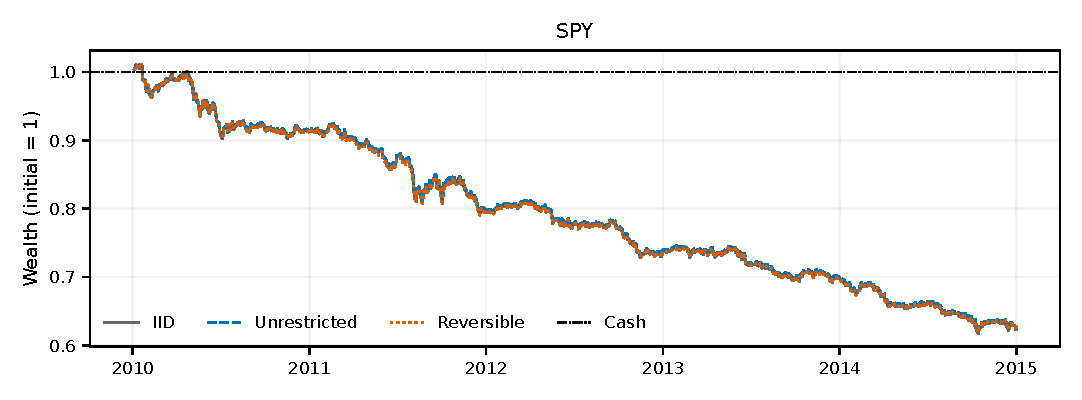
\includegraphics[width=\linewidth]{../figures/figure3.pdf}
\caption{SPY validation-period net wealth at 5 bps per side. These observations were available before the final-period protocol freeze.}\label{fig:validationwealth}
\end{figure}

\begin{figure}[!htbp]\centering
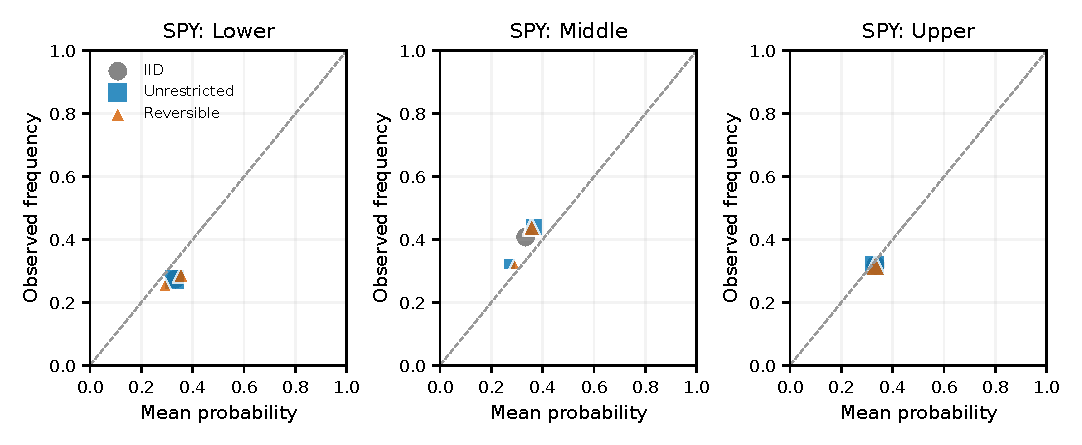
\includegraphics[width=\linewidth]{../figures/figure4.pdf}
\caption{SPY validation class-wise calibration. The same ten bins are used as in the final period; marker area increases with count.}\label{fig:validationcalibration}
\end{figure}

\clearpage
\subsection{Exposure ranges in the frozen forecasts}
\begin{table}[!htbp]\centering\small\setlength{\tabcolsep}{10pt}
\caption{Final-period exposure by model}\label{tab:weights}
\begin{tabular}{llrrr}\toprule
Asset & Model & Minimum & Maximum & Mean\\\midrule
SPY & IID & 0.499910 & 0.500000 & 0.499976\\
SPY & Unrestricted & 0.480112 & 0.520924 & 0.499531\\
SPY & Reversible & 0.470755 & 0.521767 & 0.500697\\
QQQ & IID & 0.499874 & 0.500000 & 0.499968\\
QQQ & Unrestricted & 0.478354 & 0.518332 & 0.500458\\
QQQ & Reversible & 0.473244 & 0.527278 & 0.501639\\
IWM & IID & 0.499864 & 0.500000 & 0.499966\\
IWM & Unrestricted & 0.479981 & 0.521101 & 0.499720\\
IWM & Reversible & 0.483442 & 0.512259 & 0.500618\\
\bottomrule\end{tabular}
\par\smallskip\parbox{0.98\linewidth}{\footnotesize Fractions of portfolio capital. Values are rounded from the retained descriptive summary of 2,766 final forecasts per asset. This table describes the existing allocation and does not fit an alternative rule.}
\end{table}

The mean exposures in Table~\ref{tab:weights}, before display rounding, and the mean net differences in Tables A2--A4 provide the inputs for main-text Table 6. The IID benchmark is nearly half exposure, but differences against it are not relabeled as differences against an exactly constant one-half allocation. The reconstruction described below supplies the daily records, so the fixed-half comparison, the score components of main-text Table 7 and the circulation statistics of Table 8 are computed on recorded paths rather than recovered from rounded aggregates.

\begin{table}[!htbp]\centering\footnotesize\setlength{\tabcolsep}{3pt}
\caption{Threshold and window sensitivity of the final-period comparisons}\label{tab:sensitivity}
\begin{tabular}{llrrr}\toprule
Asset & Rule & $\Delta(\mathrm U-\mathrm{IID})$ log loss & $\Delta(\mathrm R-\mathrm U)$ log loss & $\Delta$ net return (bps/day)\\
 & & [95\% CI] & [95\% CI] & [95\% CI]\\\midrule
SPY & Primary & $-$0.0053 [$-$0.0100, $-$0.0007] & $+$0.0013 [$-$0.0004, $+$0.0031] & 0.043 [$+$0.001, $+$0.087]\\
SPY & Fixed cut points & $-$0.0085 [$-$0.0137, $-$0.0035] & $+$0.0016 [$-$0.0002, $+$0.0033] & 0.045 [$+$0.003, $+$0.091]\\
SPY & Rolling 2,520 & $-$0.0048 [$-$0.0090, $-$0.0005] & $+$0.0006 [$-$0.0010, $+$0.0022] & 0.042 [$-$0.010, $+$0.099]\\
SPY & Rolling 1,260 & $-$0.0017 [$-$0.0057, $+$0.0028] & $+$0.0000 [$-$0.0020, $+$0.0021] & 0.082 [$+$0.018, $+$0.148]\\
SPY & Common start & $-$0.0054 [$-$0.0108, $+$0.0001] & $+$0.0011 [$-$0.0007, $+$0.0029] & 0.038 [$-$0.001, $+$0.079]\\
\midrule
QQQ & Primary & $-$0.0117 [$-$0.0187, $-$0.0045] & $+$0.0007 [$-$0.0004, $+$0.0017] & 0.020 [$-$0.026, $+$0.069]\\
QQQ & Fixed cut points & $-$0.0148 [$-$0.0221, $-$0.0076] & $+$0.0013 [$-$0.0001, $+$0.0026] & 0.055 [$+$0.013, $+$0.102]\\
QQQ & Rolling 2,520 & $-$0.0049 [$-$0.0098, $+$0.0003] & $+$0.0009 [$-$0.0007, $+$0.0027] & 0.115 [$+$0.021, $+$0.207]\\
QQQ & Rolling 1,260 & $-$0.0047 [$-$0.0096, $+$0.0002] & $+$0.0010 [$-$0.0008, $+$0.0029] & 0.144 [$+$0.030, $+$0.267]\\
QQQ & Common start & $-$0.0104 [$-$0.0169, $-$0.0034] & $+$0.0005 [$-$0.0005, $+$0.0016] & 0.025 [$-$0.021, $+$0.074]\\
\midrule
IWM & Primary & $-$0.0049 [$-$0.0088, $-$0.0012] & $+$0.0016 [$-$0.0001, $+$0.0034] & 0.073 [$+$0.028, $+$0.123]\\
IWM & Fixed cut points & $-$0.0043 [$-$0.0079, $-$0.0007] & $+$0.0016 [$+$0.0003, $+$0.0030] & 0.059 [$+$0.019, $+$0.104]\\
IWM & Rolling 2,520 & $-$0.0043 [$-$0.0086, $-$0.0001] & $+$0.0021 [$-$0.0006, $+$0.0048] & 0.116 [$+$0.036, $+$0.202]\\
IWM & Rolling 1,260 & $-$0.0024 [$-$0.0067, $+$0.0019] & $+$0.0015 [$-$0.0013, $+$0.0045] & 0.109 [$+$0.001, $+$0.222]\\
IWM & Common start & $-$0.0049 [$-$0.0088, $-$0.0012] & $+$0.0016 [$-$0.0001, $+$0.0034] & 0.073 [$+$0.028, $+$0.123]\\
\bottomrule\end{tabular}
\par\smallskip\parbox{0.98\linewidth}{\footnotesize U: unrestricted; R: reversible. Each rule re-estimates cut points and state counts as described in Section~\ref{sec:sensitivity}; the common-start rule applies 26 May 2000 to all three assets and leaves IWM unchanged. $\Delta$ net is the paired mean net-return difference at 5 bps per side. Intervals are percentile intervals from 5,000 paired moving blocks of length 20, conditional on the forecasts generated under each rule, without refitting and without multiplicity adjustment. Mean unrestricted levels, which are not comparable across rules, are 1.0933, 1.0732, 1.0939, 1.0969, 1.0932 for SPY and 1.0870, 1.0306, 1.0937, 1.0939, 1.0883 for QQQ under the five rules in order. Under the fixed and rolling rules the retained solver reaches a line-search precision limit at between 0.1\% and 4.6\% of estimation origins; the v13 fallback re-solves the same likelihood on simplex flow masses and accepts only positive finite fits with projected-gradient infinity norm at most $10^{-8}$. The primary rule has no fallbacks; this replaces the older softmax-gradient acceptance rule.}
\end{table}

\begin{table}[!htbp]\centering\small\setlength{\tabcolsep}{6pt}
\caption{Final-period comparisons by fixed calendar segment}\label{tab:segments}
\begin{tabular}{llrrr}\toprule
Asset & Segment & Sessions & $\Delta(\mathrm U-\mathrm{IID})$ & $\Delta(\mathrm R-\mathrm U)$\\
 & & & [95\% CI] & [95\% CI]\\\midrule
SPY & 2015--2018 & 1006 & $-$0.01182 [$-$0.01937, $-$0.00392] & $+$0.00156 [$-$0.00132, $+$0.00446]\\
SPY & 2019--2022 & 1008 & $-$0.00620 [$-$0.01295, $+$0.00153] & $+$0.00144 [$-$0.00137, $+$0.00462]\\
SPY & 2023--2025 & 752 & $+$0.00458 [$-$0.00421, $+$0.01257] & $+$0.00081 [$-$0.00268, $+$0.00433]\\
\midrule
QQQ & 2015--2018 & 1006 & $-$0.02994 [$-$0.04287, $-$0.01821] & $+$0.00075 [$-$0.00104, $+$0.00252]\\
QQQ & 2019--2022 & 1008 & $-$0.01048 [$-$0.02065, $+$0.00006] & $+$0.00085 [$-$0.00058, $+$0.00252]\\
QQQ & 2023--2025 & 752 & $+$0.01106 [$+$0.00239, $+$0.02182] & $+$0.00038 [$-$0.00189, $+$0.00247]\\
\midrule
IWM & 2015--2018 & 1006 & $-$0.00793 [$-$0.01358, $-$0.00167] & $+$0.00283 [$+$0.00023, $+$0.00538]\\
IWM & 2019--2022 & 1008 & $-$0.00556 [$-$0.01226, $+$0.00150] & $+$0.00102 [$-$0.00211, $+$0.00408]\\
IWM & 2023--2025 & 752 & $-$0.00011 [$-$0.00696, $+$0.00649] & $+$0.00071 [$-$0.00312, $+$0.00438]\\
\bottomrule\end{tabular}
\par\smallskip\parbox{0.98\linewidth}{\footnotesize Segment boundaries were fixed for this revision and are exploratory. Each interval is a percentile interval from 5,000 paired moving blocks of length 20 computed within the segment, conditional on the saved forecasts and without refitting. Nine segment-specific intervals are not a segment-difference test; adjacent segments share no sessions but the point estimates are not independent of the full-period result.}
\end{table}


\begin{table}[!htbp]\centering\footnotesize\setlength{\tabcolsep}{3pt}
\caption{Expected cost of imposing detailed balance in the controlled simulation}\label{tab:simulation}
\setlength{\tabcolsep}{3pt}\begin{tabular}{lrrrrrr}\toprule
Process & $j$ & $n=250$ & $n=500$ & $n=1{,}260$ & $n=2{,}520$ & $n=5{,}000$\\\midrule
Reversible truth ($j=0$) & +0.0 & -2.087 (0.137) & -1.008 (0.062) & -0.431 (0.027) & -0.214 (0.013) & -0.101 (0.006)\\
Weak circulation ($j=-0.7$) & -0.7 & -1.626 (0.132) & -0.661 (0.061) & -0.061 (0.026) & +0.132 (0.013) & +0.245 (0.007)\\
Fitted magnitude ($j=-1.4$) & -1.4 & -0.638 (0.134) & +0.374 (0.072) & +0.950 (0.023) & +1.165 (0.012) & +1.257 (0.007)\\
\bottomrule\end{tabular}
\par\smallskip\parbox{0.98\linewidth}{\footnotesize Entries are $10^{3}$ times the difference in expected log loss between the restricted and unrestricted estimators, evaluated against the generating matrix; Monte Carlo standard errors are in parentheses, from 500 simulated chains per cell. $j$ is the circulation $J_{12}=J_{23}=J_{31}$ in percentage points of daily flow. Positive values mean that imposing detailed balance costs expected log loss. The generating matrices have a uniform stationary distribution, baseline transition probabilities of 0.35 on the diagonal and 0.325 off the diagonal; stationary flows are one-third of those probabilities. The design was fixed after the empirical results were seen and is calibrated to them, so the agreement reported in Section~\ref{sec:simulation} is an explanation, not a confirmation.}
\end{table}


\begin{table}[!htbp]\centering\small\setlength{\tabcolsep}{8pt}
\caption{Calibration bin occupancy in the final period}\label{tab:bins}
\begin{tabular}{llrrr}\toprule
Asset & Model & Empty bins (of 30) & Smallest non-empty & Largest\\\midrule
SPY & IID & 27 & 2766 & 2766\\
SPY & Unrestricted & 25 & 2 & 2766\\
SPY & Reversible & 25 & 826 & 2766\\
\midrule
QQQ & IID & 27 & 2766 & 2766\\
QQQ & Unrestricted & 23 & 201 & 2565\\
QQQ & Reversible & 24 & 805 & 2766\\
\midrule
IWM & IID & 27 & 2766 & 2766\\
IWM & Unrestricted & 25 & 670 & 2766\\
IWM & Reversible & 25 & 78 & 2766\\
\bottomrule\end{tabular}
\par\smallskip\parbox{0.98\linewidth}{\footnotesize Bins are the ten fixed edges of Figure~\ref{fig:calibration}, counted separately for each of the three one-versus-rest classes, so thirty bins are possible. Most are empty: the forecast probabilities concentrate near one third, and a bin holding two observations provides little precision about calibration. The counts here are the only measure of how much support each plotted marker has; the summary statistic and reference diagnostic built from the same bins are in Table~\ref{tab:calibration}.}
\end{table}


\subsection{Secondary families and calibration}\label{app:families}
Table~\ref{tab:jointbrier} applies the same stepdown procedure to the six Brier-score contrasts. Here QQQ and IWM both survive, with adjusted $p$-values of 0.006 and 0.041, and SPY does not (0.067). The Brier family is adjusted within itself: its $p$-values do not provide joint error control with Table~\ref{tab:joint}, and the difference between the two score families is a difference in how the scores weight errors, not a contradiction. For log loss, QQQ is significant across the reported correction methods and IWM is significant only under stepdown. The two score families should therefore be identified explicitly whenever significance is summarized.

Table~\ref{tab:jointecon} applies the procedure to one exploratory family of twelve economic contrasts: six mean net-return differences and six Sharpe differences, all at 5 basis points per side. Four Sharpe contrasts survive. SPY and IWM gain on unrestricted minus IID (adjusted $p=0.032$ and $0.001$) and lose on reversible minus unrestricted (0.006 and 0.007, with negative estimates, that is, against the restricted model). Among mean net returns only IWM's unrestricted advantage survives (0.022); its reversible contrast falls just outside (0.054), and the SPY and QQQ net contrasts do not survive (0.184 and 0.555). The family inherits the allocation rule and the cost scenario, and no power claim is made for it.

Table~\ref{tab:calibration} reports the observed count-weighted calibration error and a percentile interval from resampling forecast--outcome pairs in moving blocks. It also retains a separate simulation diagnostic: with all saved forecasts held fixed, 500 independent outcome sequences are drawn, each day from its forecast vector. The reported tail fraction is $(1+K)/501$, where $K$ counts simulated errors at least as large as the observed error. Its minimum attainable value is approximately 0.002. All nine values are at most 0.004 under this reference model, without adjustment across the nine diagnostics.

This simulation assumes more than bin-level or sequential calibration. In an adaptive forecasting system, later probabilities depend on earlier outcomes; independently resampling outcomes while freezing the entire probability sequence does not regenerate that dependence. These tail fractions are consequently reported as reference-model diagnostics, not as a generally valid rejection of calibration under serial dependence or regime change. The block-bootstrap intervals and the independent-draw reference distribution also answer different questions; a positive percentile lower bound for this nonnegative error statistic is not itself a calibrated test of zero error.

Realized final-period class frequencies are 29.9/37.3/32.9\% for SPY, 29.1/39.2/31.6\% for QQQ and 32.8/36.7/30.6\% for IWM (rounding can affect the sums). Historical terciles do not force these future frequencies to equal one-third. This imbalance is consistent with a marginal discrepancy for the nearly uniform IID forecast, but comparison with one-third alone cannot attribute the diagnostic for the time-varying Markov forecasts. Marginal calibration compares mean forecast probabilities with realized frequencies; conditional calibration requires more information. Only three to seven class--bin cells contain at least thirty observations, limiting detailed interpretation of the reliability curves.

\begin{table}[!htbp]\centering\small\setlength{\tabcolsep}{6pt}
\caption{Brier-score contrasts, adjusted within their own family}\label{tab:jointbrier}
\footnotesize\begin{tabular}{llrrrr}\toprule
Asset & Contrast & Estimate & Pointwise 95\% CI & Romano--Wolf $p$ & Holm $p$\\\midrule
SPY & $\mathrm{U}-\mathrm{IID}$ & $-$0.003737 & [$-$0.006875, $-$0.000653] & 0.067 & 0.066\\
SPY & $\mathrm{R}-\mathrm{U}$ & $+$0.000999 & [$-$0.000141, $+$0.002195] & 0.190 & 0.230\\
QQQ & $\mathrm{U}-\mathrm{IID}$ & $-$0.008222 & [$-$0.013047, $-$0.003308] & 0.006 & 0.010\\
QQQ & $\mathrm{R}-\mathrm{U}$ & $+$0.000564 & [$-$0.000087, $+$0.001199] & 0.190 & 0.230\\
IWM & $\mathrm{U}-\mathrm{IID}$ & $-$0.003356 & [$-$0.005981, $-$0.000856] & 0.041 & 0.045\\
IWM & $\mathrm{R}-\mathrm{U}$ & $+$0.001031 & [$-$0.000081, $+$0.002179] & 0.190 & 0.230\\
\bottomrule\end{tabular}
\par\smallskip\parbox{0.98\linewidth}{\footnotesize Separate family, adjusted within itself only. Estimates are model minus IID for the first contrast and reversible minus unrestricted for the second; for scores a negative difference favours the first model, for returns a positive difference does. Intervals are pointwise percentile intervals from the same 5,000 paired moving-block draws, reindexed jointly across the six contrasts; the $p$-values are stepdown-adjusted within this family and do not control errors jointly with Table~\ref{tab:joint}.}
\end{table}


\begin{table}[!htbp]\centering\small\setlength{\tabcolsep}{5pt}
\caption{Economic contrasts, adjusted within their own family}\label{tab:jointecon}
\footnotesize\begin{tabular}{llrrrr}\toprule
Asset & Contrast & Estimate & Simultaneous 95\% CI & Romano--Wolf $p$ & Holm $p$\\\midrule
\multicolumn{6}{l}{\emph{Mean net return, 5 bps per side (bps/day)}}\\
\addlinespace[2pt]
SPY & $\mathrm{U}-\mathrm{IID}$ & $+$0.0425 & [$-$0.0172, $+$0.1022] & 0.184 & 0.326\\
SPY & $\mathrm{R}-\mathrm{U}$ & $-$0.0359 & [$-$0.0924, $+$0.0206] & 0.220 & 0.407\\
QQQ & $\mathrm{U}-\mathrm{IID}$ & $+$0.0200 & [$-$0.0456, $+$0.0856] & 0.555 & 1.000\\
QQQ & $\mathrm{R}-\mathrm{U}$ & $-$0.0150 & [$-$0.0605, $+$0.0306] & 0.555 & 1.000\\
IWM & $\mathrm{U}-\mathrm{IID}$ & $+$0.0728 & [$+$0.0059, $+$0.1396] & 0.022 & 0.040\\
IWM & $\mathrm{R}-\mathrm{U}$ & $-$0.0688 & [$-$0.1420, $+$0.0043] & 0.054 & 0.063\\
\midrule
\multicolumn{6}{l}{\emph{Sharpe ratio (conventional $\sqrt{252}$ scaling)}}\\
\addlinespace[2pt]
SPY & $\mathrm{U}-\mathrm{IID}$ & $+$0.0227 & [$+$0.0006, $+$0.0447] & 0.032 & 0.048\\
SPY & $\mathrm{R}-\mathrm{U}$ & $-$0.0252 & [$-$0.0457, $-$0.0047] & 0.006 & 0.009\\
QQQ & $\mathrm{U}-\mathrm{IID}$ & $+$0.0041 & [$-$0.0137, $+$0.0219] & 0.555 & 1.000\\
QQQ & $\mathrm{R}-\mathrm{U}$ & $-$0.0060 & [$-$0.0193, $+$0.0073] & 0.369 & 0.881\\
IWM & $\mathrm{U}-\mathrm{IID}$ & $+$0.0278 & [$+$0.0085, $+$0.0470] & 0.001 & 0.002\\
IWM & $\mathrm{R}-\mathrm{U}$ & $-$0.0251 & [$-$0.0459, $-$0.0044] & 0.007 & 0.009\\
\bottomrule\end{tabular}
\par\smallskip\parbox{0.98\linewidth}{\footnotesize One exploratory family of twelve contrasts, adjusted within itself, with no joint error control across this family and Table~\ref{tab:joint}. Estimates are unrestricted minus IID for the first contrast and reversible minus unrestricted for the second; for both metrics a positive difference favours the first model. Intervals are simultaneous, from the single-step max-$|t|$ critical value of 2.721; the $p$-values are stepdown-adjusted. The Sharpe statistic is recomputed inside every bootstrap draw from the resampled days, so its sampling variability is that of a ratio rather than of a mean.}
\end{table}


\begin{table}[!htbp]\centering\small\setlength{\tabcolsep}{6pt}
\caption{Observed calibration error and independent-draw reference diagnostic}\label{tab:calibration}
\begin{tabular}{llrrrr}\toprule
Asset & Model & Observed error & 95\% CI & Reference $p$ & Bins with $n\ge30$\\\midrule
SPY & IID & 0.0264 & [0.0117, 0.0469] & 0.002 & 3\\
SPY & Unrestricted & 0.0239 & [0.0116, 0.0429] & 0.002 & 4\\
SPY & Reversible & 0.0242 & [0.0149, 0.0434] & 0.002 & 5\\
\midrule
QQQ & IID & 0.0394 & [0.0198, 0.0613] & 0.002 & 3\\
QQQ & Unrestricted & 0.0363 & [0.0201, 0.0555] & 0.002 & 7\\
QQQ & Reversible & 0.0345 & [0.0194, 0.0536] & 0.002 & 6\\
\midrule
IWM & IID & 0.0223 & [0.0086, 0.0421] & 0.004 & 3\\
IWM & Unrestricted & 0.0213 & [0.0097, 0.0396] & 0.004 & 5\\
IWM & Reversible & 0.0229 & [0.0103, 0.0413] & 0.002 & 5\\
\bottomrule\end{tabular}
\par\smallskip\parbox{0.98\linewidth}{\footnotesize The statistic is the mean over the three one-versus-rest classes of $\sum_b (n_b/N)\lvert\bar p_b-\hat o_b\rvert$ over the ten fixed bins of Figure~\ref{fig:calibration}. The interval is a percentile interval from 5,000 paired moving blocks of length 20 computed by resampling days and recomputing every bin. The reference $p$ uses 500 simulations with independent outcomes drawn from each day's frozen forecast and the plus-one correction. It is a diagnostic under that stronger reference model, not a general sequential-calibration test; values are not adjusted across the nine rows. The minimum possible value is $1/501$. Three to seven of the thirty possible bins hold thirty or more observations, so the statistic is dominated by a few cells.}
\end{table}


\clearpage
\subsection{Benchmark layers, closed-form references and conditional returns}\label{app:layers}
Tables~\ref{tab:layerrules}--\ref{tab:statemeans} support Sections~\ref{sec:layers}, \ref{sec:circulation}, \ref{sec:economics} and \ref{sec:simulation}. They are computed from the saved forecasts and price inputs of the v13 run and the four rule panels of Table~\ref{tab:sensitivity}, without refitting the IID, unrestricted or reversible models. The V and M benchmarks are refitted at each origin from the same labelled history. All of these analyses were specified after the primary results and are exploratory.

\begin{table}[!htbp]\centering\footnotesize\setlength{\tabcolsep}{2pt}
\caption{Benchmark layers under the threshold and window rules}\label{tab:layerrules}
\begin{tabular}{llrrrrr}\toprule
Asset & Rule & V share & $|w^{\mathrm V}-\tfrac12|$ & Direction & Weighted direction & Direction net\\
 & & (\%) & & ($10^{-3}$ nats) & ($10^{-3}$) & (bps/day)\\\midrule
SPY & Primary & 82 & 0.00002 & $+$0.04 [$-$1.04, $+$1.05] & $-$0.77 [$-$2.29, $+$0.65] & $+$0.043 [$+$0.001, $+$0.087]\\
SPY & Fixed & 77 & 0.01322 & $+$0.32 [$-$0.73, $+$1.30] & $-$0.68 [$-$2.14, $+$0.64] & $+$0.038 [$-$0.000, $+$0.082]\\
SPY & Roll 2,520 & 89 & 0.00014 & $+$0.28 [$-$1.23, $+$1.74] & $-$0.63 [$-$2.72, $+$1.28] & $+$0.042 [$-$0.010, $+$0.098]\\
SPY & Roll 1,260 & 108 & 0.00026 & $-$0.41 [$-$2.29, $+$1.46] & $-$1.96 [$-$4.45, $+$0.36] & $+$0.082 [$+$0.018, $+$0.148]\\
\midrule
QQQ & Primary & 82 & 0.00003 & $-$0.07 [$-$1.12, $+$1.00] & $-$0.14 [$-$1.47, $+$1.12] & $+$0.020 [$-$0.026, $+$0.069]\\
QQQ & Fixed & 79 & 0.01376 & $-$0.22 [$-$1.13, $+$0.68] & $-$0.77 [$-$1.93, $+$0.33] & $+$0.043 [$+$0.002, $+$0.089]\\
QQQ & Roll 2,520 & 56 & 0.00014 & $-$0.43 [$-$2.17, $+$1.50] & $-$1.92 [$-$4.41, $+$0.69] & $+$0.115 [$+$0.021, $+$0.207]\\
QQQ & Roll 1,260 & 56 & 0.00026 & $-$0.54 [$-$2.88, $+$1.73] & $-$1.97 [$-$5.24, $+$1.07] & $+$0.144 [$+$0.030, $+$0.267]\\
\midrule
IWM & Primary & 66 & 0.00003 & $-$1.31 [$-$2.41, $-$0.24] & $-$1.44 [$-$2.65, $-$0.29] & $+$0.073 [$+$0.028, $+$0.123]\\
IWM & Fixed & 73 & 0.00269 & $-$0.78 [$-$1.70, $+$0.10] & $-$1.24 [$-$2.35, $-$0.25] & $+$0.058 [$+$0.018, $+$0.103]\\
IWM & Roll 2,520 & 56 & 0.00014 & $-$1.76 [$-$3.66, $+$0.06] & $-$2.18 [$-$4.38, $-$0.11] & $+$0.116 [$+$0.036, $+$0.202]\\
IWM & Roll 1,260 & 69 & 0.00026 & $-$0.66 [$-$3.17, $+$1.75] & $-$1.12 [$-$4.12, $+$1.77] & $+$0.109 [$+$0.001, $+$0.222]\\
\bottomrule\end{tabular}
\par\smallskip\parbox{0.98\linewidth}{\footnotesize V share is $(\bar\ell^{\mathrm V}-\bar\ell^{\mathrm{IID}})/(\bar\ell^{\mathrm U}-\bar\ell^{\mathrm{IID}})$ in percent. The second column is the mean of $|w^{\mathrm V}_t-\tfrac12|$. The direction column, $\mathrm{U}-\mathrm{M}$, is the paired difference in the conditional upper-versus-lower term of Equation~\eqref{eq:scorefactor}; it equals the total $\mathrm{U}-\mathrm{M}$ log-loss difference. The weighted column multiplies that term on each outer-tercile day by $|r_{t+1}|$ divided by the mean of $|r_{t+1}|$ over outer-tercile days; it is a magnitude-weighted diagnostic, not a proper score for the tercile event. Net returns use 5 bps per side. Each rule labels history with its own cut points, as in Table~\ref{tab:sensitivity}. Under fixed cut points the marginal upper share departs from one-half, so V, M and IID all carry a common tilt. Intervals are pointwise percentile intervals from 5,000 paired moving blocks of length 20 without refitting; rows share sessions and assets.}
\end{table}


\begin{table}[!htbp]\centering\footnotesize\setlength{\tabcolsep}{3pt}
\caption{Closed-form reference for the cost of detailed balance}\label{tab:restriction}
\resizebox{\linewidth}{!}{\begin{tabular}{lrrrrrrr}\toprule
\multicolumn{8}{l}{\emph{Panel A. Final-period reference values ($10^{-3}$ nats unless stated)}}\\
Asset & Mean $j_t$ (pp) & Mean $D_t$ & Mean $1/(2n_t)$ & Fitted reference & Frozen $j$ (pp) & Frozen reference & Observed $\mathrm{R}-\mathrm{U}$ [95\% CI]\\\midrule
SPY & $-$1.40 & 1.363 & 0.073 & 1.289 & $-$1.29 & 1.087 & $+$1.315 [$-$0.422, $+$3.131]\\
QQQ & $-$0.77 & 0.450 & 0.095 & 0.355 & $-$0.96 & 0.564 & $+$0.685 [$-$0.358, $+$1.681]\\
IWM & $-$1.32 & 1.232 & 0.102 & 1.131 & $-$1.04 & 0.650 & $+$1.595 [$-$0.140, $+$3.359]\\
\bottomrule\end{tabular}}

\medskip
\resizebox{\linewidth}{!}{\begin{tabular}{lrrrrrr}\toprule
\multicolumn{7}{l}{\emph{Panel B. Controlled simulation: closed form / Monte Carlo ($10^{-3}$ nats)}}\\
Process & $n^\ast$ & $n=250$ & $n=500$ & $n=1{,}260$ & $n=2{,}520$ & $n=5{,}000$\\\midrule
Reversible truth ($j=0$) & --- & $-$2.000 / $-$2.087 & $-$1.000 / $-$1.008 & $-$0.397 / $-$0.431 & $-$0.198 / $-$0.214 & $-$0.100 / $-$0.101\\
Weak circulation ($j=-0.7$) & 1,474 & $-$1.661 / $-$1.626 & $-$0.661 / $-$0.661 & $-$0.058 / $-$0.061 & $+$0.141 / $+$0.132 & $+$0.239 / $+$0.245\\
Fitted magnitude ($j=-1.4$) & 368 & $-$0.642 / $-$0.638 & $+$0.358 / $+$0.374 & $+$0.961 / $+$0.950 & $+$1.159 / $+$1.165 & $+$1.258 / $+$1.257\\
\bottomrule\end{tabular}}
\par\smallskip\parbox{0.98\linewidth}{\footnotesize $D_t=\sum_{ij}F_{ij}\log(F_{ij}/S_{ij})$ with $F=\operatorname{diag}(\pi)\hat P_t$ and $S=(F+F^\top)/2$, computed from the smoothed unrestricted matrix at each origin; $n_t$ is the number of historical transitions. The fitted reference averages $D_t-1/(2n_t)$ over origins and uses matrices that incorporate earlier final-period outcomes. The frozen reference uses only the matrix of the first final-period origin (history through 31 December 2014) and the mean of $1/(2n_t)$. Both are first-order references under a stationary chain, not tests, and neither models the updating cut points. Observed values and intervals repeat Table~\ref{tab:intervals}. In Panel B, $n^\ast=1/(2D)$ is the approximate crossover length, and Monte Carlo values repeat Table~\ref{tab:simulation}; the largest absolute difference is 1.27 Monte Carlo standard errors.}
\end{table}


\begin{table}[!htbp]\centering\footnotesize\setlength{\tabcolsep}{4pt}
\caption{Rolling class-frequency forecasts under the primary cut points}\label{tab:rollfreq}
\begin{tabular}{lrrrrrr}\toprule
Asset & Window & $\mathrm{Roll}-\mathrm{IID}$ & $\mathrm{U}-\mathrm{Roll}$ & \multicolumn{3}{c}{$\mathrm{U}-\mathrm{Roll}$ by segment}\\
 & (sessions) & [95\% CI] & [95\% CI] & 2015--2018 & 2019--2022 & 2023--2025\\\midrule
SPY & 252 & $-$14.44 [$-$30.85, $+$0.47] & $+$9.13 [$-$5.01, $+$24.94] & $+$28.17 & $+$0.72 & $-$5.08\\
SPY & 504 & $-$9.40 [$-$23.56, $+$3.42] & $+$4.09 [$-$8.04, $+$17.90] & $+$12.13 & $+$4.68 & $-$7.48\\
SPY & 1,260 & $-$8.14 [$-$20.34, $+$3.20] & $+$2.82 [$-$7.97, $+$14.49] & $+$22.94 & $-$19.73 & $+$6.14\\
\midrule
QQQ & 252 & $-$21.88 [$-$40.83, $-$4.78] & $+$10.18 [$-$4.26, $+$26.54] & $+$29.45 & $-$2.53 & $+$1.44\\
QQQ & 504 & $-$17.33 [$-$35.26, $-$1.32] & $+$5.63 [$-$8.51, $+$21.13] & $+$15.12 & $+$1.74 & $-$1.85\\
QQQ & 1,260 & $-$11.25 [$-$28.53, $+$4.35] & $-$0.45 [$-$14.05, $+$14.45] & $+$26.61 & $-$32.55 & $+$6.38\\
\midrule
IWM & 252 & $-$7.37 [$-$19.65, $+$3.67] & $+$2.43 [$-$8.29, $+$14.16] & $+$16.28 & $-$5.75 & $-$5.14\\
IWM & 504 & $-$6.72 [$-$17.54, $+$2.59] & $+$1.78 [$-$7.52, $+$12.22] & $+$14.50 & $-$4.21 & $-$7.21\\
IWM & 1,260 & $-$4.03 [$-$13.19, $+$4.48] & $-$0.91 [$-$9.41, $+$7.97] & $+$20.82 & $-$20.34 & $-$3.93\\
\bottomrule\end{tabular}
\par\smallskip\parbox{0.98\linewidth}{\footnotesize Log-loss differences in $10^{-3}$ nats; negative values favour the first model. The rolling forecast uses the smoothed frequencies of the most recent $W$ historical labels, relabelled with the cut points of the primary rule at each origin, and no state dependence. Window lengths were chosen after the primary results were known. Intervals are pointwise percentile intervals from 5,000 paired moving blocks of length 20; segment intervals are in the replication results.}
\end{table}


\begin{table}[!htbp]\centering\footnotesize\setlength{\tabcolsep}{5pt}
\caption{Unrestricted exposure and next-session return by current state}\label{tab:statemeans}
\begin{tabular}{llrrrr}\toprule
Asset & Current state & Mean $w^{\mathrm U}$ (\%) & Mean $r_{t+1}$ (bps) & Pointwise 95\% CI & Simultaneous 95\% CI\\\midrule
SPY & Lower & 51.668 & $+$7.61 & [$+$1.73, $+$14.75] & [$-$1.62, $+$16.84]\\
SPY & Middle & 49.824 & $-$0.23 & [$-$4.25, $+$3.61] & [$-$5.72, $+$5.26]\\
SPY & Upper & 48.541 & $-$0.36 & [$-$5.34, $+$4.60] & [$-$7.32, $+$6.61]\\
\midrule
QQQ & Lower & 50.281 & $+$13.37 & [$+$5.73, $+$22.53] & [$+$1.68, $+$25.05]\\
QQQ & Middle & 51.040 & $+$0.89 & [$-$4.50, $+$6.26] & [$-$6.67, $+$8.45]\\
QQQ & Upper & 48.596 & $-$4.66 & [$-$12.51, $+$2.90] & [$-$15.39, $+$6.06]\\
\midrule
IWM & Lower & 51.503 & $+$7.64 & [$+$0.65, $+$16.14] & [$-$3.25, $+$18.53]\\
IWM & Middle & 48.743 & $-$6.38 & [$-$12.08, $-$0.72] & [$-$14.31, $+$1.55]\\
IWM & Upper & 49.805 & $-$4.68 & [$-$12.89, $+$3.55] & [$-$16.26, $+$6.91]\\
\bottomrule\end{tabular}
\par\smallskip\parbox{0.98\linewidth}{\footnotesize Final-period descriptive summaries by the state of the origin session under the primary rule. Intervals resample sessions with the common moving blocks and recompute each conditional mean as a ratio of resampled sums; the simultaneous interval uses the single-step max-$|t|$ critical value 2.750 over the nine cells. These are conditional averages over the evaluation period, not a trading rule; selecting states from them and reporting returns in the same period would be in-sample.}
\end{table}


\clearpage
\section{Computational verification and limitations}
The v13 reproduction record reports a full run from locally retained reconstructed prices through forecasts, sensitivity analyses, simulation, figures, tables and 231 aggregate comparisons. This revision checked the existing run artifacts: all three forecast hashes match the recorded values, the ten v13 generated tables match their shipped counterparts, and the aggregate verification returns zero mismatches. These are internal reproducibility checks on specified inputs; they do not establish that an external download is bit-identical. The present revision additionally recomputed the SPY Sharpe moments and their exact accounting decomposition. It did not launch another complete pipeline run or repeat the separate independent-optimizer experiment reported below. Revision v16 adds the benchmark layers and closed-form references of Appendix~\ref{app:layers}. They recompute labels, cut points and unrestricted forecasts from the same price inputs, match every saved target label and every saved unrestricted forecast to within $10^{-16}$, and verify Equation~\eqref{eq:halfbound} at every origin of the primary and rolling rules. The v16 revision did not rerun the frozen package or the full pipeline.

The original estimator archive is unchanged. In the v13 sensitivity implementation, a failed original fit triggers simplex optimization of the same likelihood followed by stationarity-equation polishing, with a projected-gradient acceptance ceiling of $10^{-8}$. The older softmax-gradient ceiling is no longer the fallback rule. This numerical change does not supply evidence about bootstrap coverage.

The original analysis used Python 3.12.6, NumPy 2.3.2, pandas 2.3.3, SciPy 1.18.1,
yfinance 1.8.0 and exchange\_calendars 4.13.2. State cutpoints are recomputed only
from information available at each origin. Missing, duplicate, invalid or
non-finite price records are rejected; calendar coverage is checked separately.

The supplied verification record describes fifteen synthetic checks covering a reversible cycle with a known analytic solution,
sparse and random count histories, future-data perturbation, known scoring and
drawdown values, invalid data, command-line integration, calendar gaps, bootstrap
block structure, identical-model contrasts, reproducibility, short samples and
undefined Sharpe comparisons. That record reports that a fresh environment reproduced the saved SPY
validation forecasts, calibration, numeric summaries and bootstrap comparisons
exactly. This is a validation-period refit, not a claim of a separate exact refit
of every final run.

The supplied record also reports a separate arithmetic audit of all 8,298 asset/target records in the final
period. It reconciled origin-specific historical thresholds, next-session timing,
target labels, probabilities, weights, turnover, costs, scores, portfolio metrics
and calibration with absolute and relative tolerances of $10^{-12}$.
Source and evidence fingerprints matched. All saved reversible fits reported
convergence; the maximum detailed-balance residual was
$2.7755575615628914\times10^{-17}$. The detailed-balance residual checks feasibility of a constraint imposed by the parameterization; it does not by itself establish numerical optimality. An independent estimator and multi-start comparison are reported below. These checks also do not establish bootstrap coverage under structural change.

Earlier revisions added exact score and daily-return identities, exposure summaries from the retained descriptive audit, and arithmetic transformations of reported aggregate estimates. The cost-only illustration and main-text Table 6 can be regenerated with the accompanying arithmetic script, \texttt{recompute.py}, in the \texttt{revision\_audit} directory. Those arithmetic checks alone did not rerun market-data estimation. The reconstruction reported below does rerun it, on a freshly retrieved panel, and reproduces the published final-period forecasts to the precision described there.

Exact probability-bin replication uses round-trip floating-point parsing.
Otherwise, a decimal value at a bin boundary can move across the boundary after
CSV parsing. This verification detail does not alter the frozen model or outputs.

Only code, documentation and cryptographic fingerprints are prepared for public
release. Raw or normalized prices, realized daily returns, daily forecasts and
local audit logs are excluded from that package. The original data remain subject
to third-party terms; the software license of a retrieval library is not a license
to redistribute market data. A new authorized download may not match the archived
snapshot, and a different licensed source constitutes a new data version.

The retained timestamps and hashes document the internal sequence of analysis. The design-freeze and retrospective-analysis limitations are stated in Sections~\ref{sec:design} and 5.

\subsection{Reconstructed panel and independent estimator}\label{app:reconstruction}
The archived snapshot is not distributed. To test whether the published estimates depend on that particular file, the panel was rebuilt from a fresh retrieval of the same public vendor series, using the adjustment convention of the original adapter, and the unmodified package was rerun. Record counts (8,288, 6,746 and 6,438 through 31 December 2025) and first and last dates match the stored fingerprint, while the normalized-file hashes differ. Historical vendor revisions are a possible explanation; the supplied records do not isolate their contribution. Table~\ref{tab:repro} compares the resulting final-period estimates with the published ones.

A common multiplicative adjustment to a session's open and close leaves its return, and therefore return-based cut points, unchanged. A revision that changes $C/O$ can instead alter historical quantiles, state labels and transition counts. For QQQ, the supplied reconstruction reports two of the 2,766 target returns within $10^{-5}$ of an origin-specific cut point and none within $10^{-6}$. This proximity check does not bound how many historical labels changed. Nor does agreement in IID log loss to six decimals establish label agreement, because the IID forecast is nearly uniform. The unrestricted-minus-IID difference changes in the sixth decimal. Without the archived panel, the affected records and the precise cause of the difference cannot be identified.

\begin{table}[!htbp]\centering\small\setlength{\tabcolsep}{7pt}
\caption{Reproduction against the published final-period estimates}\label{tab:repro}
\begin{tabular}{lrrrrr}\toprule
Asset & Records & Final $N$ & IID log loss & IID log loss & $\mathrm{U}-\mathrm{IID}$\\
 & & & (published) & (reconstructed) & (published / reconstructed)\\\midrule
SPY & 8,288 & 2,766 & 1.098647 & 1.098647 & $-$0.005314 / $-$0.005314\\
QQQ & 6,746 & 2,766 & 1.098673 & 1.098673 & $-$0.011697 / $-$0.011699\\
IWM & 6,438 & 2,766 & 1.098647 & 1.098647 & $-$0.004942 / $-$0.004942\\
\bottomrule\end{tabular}
\par\smallskip\parbox{0.98\linewidth}{\footnotesize U: unrestricted. The reconstructed column applies the frozen code to the rebuilt panel without modification. The QQQ difference is $2\times10^{-6}$; the supplied records do not identify its record-level cause; no target return lies within $10^{-6}$ of a cut point at its origin and the signed conclusions are unchanged. The realized open-to-close returns that the models classify are invariant to a same-session adjustment factor, so differing price-file hashes need not imply different intraday returns.}
\end{table}

The reversible estimator was also reimplemented independently. The smoothed likelihood was written in the six flow masses and optimized directly on the simplex by sequential quadratic programming with numerical gradients, in contrast to the softmax parameterization, analytic gradient and BFGS of the retained code. At all 2,766 final-period origins per asset the two solutions agree to $|\Delta\,\text{NLL}|\le7.3\times10^{-12}$ and $|\Delta P|\le2.2\times10^{-8}$ in every fitted entry. Ten random starts per origin, at every twenty-fifth origin, never improved on the retained fit by more than $1.8\times10^{-12}$ nats. The retained fits are therefore taken as numerical optima of the stated objective, without claiming global optimality for the parameterization as such.

Component losses and circulation flows are computed from the reconstructed daily records. Their intervals use the same paired moving-block design, seed and block length as the total-loss intervals, recomputed on component series without refitting. No bootstrap is applied to the circulation path itself, whose first-order autocorrelation of 0.99 makes a short-block interval uninformative; the path is reported descriptively. These additions recompute the diagnostics on the rebuilt panel rather than replaying the archived snapshot.

The roles of the generative AI systems used for data reconstruction, code,
analysis and text are listed by system in the Declaration of Generative AI in
Scientific Writing of the main text.
